% Hreyfilýsing
\section{Hreyfilýsing í einni vídd}
% position time
Þegar hlutir hreyfast í tíma og rúmi notum við oftast staðsetningu og breytingu
á staðsetningu hluta til að lýsa því hvernig við aukum hraða, hversu hratt
hraðinn breytist og sambærilegar hugmyndir.

% speed, acceleration
Staðsetning er oft táknuð með $\ulengthx$ eða $\ulengths$, og tími er táknaður 
með $t$. Meðalhraði er skilgreindur til að vera
\begin{equation}
	\uspeed
		\equiv \frac{\Delta\ulengths}{\Delta\utime}
		= \frac{\ulengths_2 - \ulengths_1}{\utime_2 - \utime_1}
\end{equation}
þar sem $\uspeed$ táknar hraða. Þar sem $\Delta$ táknar breytingu á staðsetningu
og tíma. Þá er hægt að segja hraði er breyting á staðsetningu á meðan breyting í
tíma á sér stað. Fyrir lengra komna er augnarblikshraði gefinn við
\begin{align}
	v = \lim_{\Delta \utime \to 0} 
		\frac{ \Delta \ulengths }{ \Delta \utime} = \frac{ds}{dt}
\end{align}
%
\marginpar{
		  Markgildi eru táknuð með 
		  $\lim$ og eru mikið notuð í stærðfræðigreiningu (calculus) 
		  og henta til að skoða breytingu á föllum. Hérna er
		  vegalengd, hraði og hröðun föll af tíma. 
		  }
%
þegar $\Delta \utime \to 0$ þá er tímabilið sem færslan $\Delta \ulengths$ gerist
yfir að verða eins lítið eins og hægt er. Hins vegar mun það aldrei ná að verða núll,
en verður eins lítið og mögulegt er. Það verður ekki farið dýpra í þess útlistun
sem stendur en smæðar reikningur verður tekinn fyrir seinna í námsefninu.


Meðalhröðun er skilgreind til að vera breyting í hraða yfir tíma, sem gefur
\begin{equation}
	\uaccelea \equiv \frac{\Delta\uspeed}{\Delta\utime}
		= \frac{\uspeed_2 - \uspeed_1}{\utime_2 - \utime_1}
\end{equation}
og hérna táknar $\uaccelea$ hröðunina, sem er hversu stór hraðabreytingin er
á hverja tímaeiningu. Í raun er núna búið að skilgreina allt sem er þörf á, 
afgangurinn af vinnunni er að finna not og beita jöfnunum. Hlutur undir hröðun
breytir hraða sínum með
\begin{equation}
	\uspeed_\text{loka} = \uspeed_\text{byrjun} + \uaccelea \Delta\utime
\end{equation}
aftur á móti þegar hraði breytist er vegalengdin sem er farin flóknari að finna.
Til þess getum við nýtt hraða-tíma gröf sem verða tekin fyrir nánar í hluta
~\ref{sec:motion:speedtime}.
Augnablikshröðun er gefinn við
\begin{align}
	v = \lim_{\Delta \utime \to 0} 
		\frac{ \Delta \uaccelea }{ \Delta \utime} = \frac{dv}{dt}
\end{align}
sem myndi lýsa hröðuninni á hverju augnabliki fyrir hraðafall.

%
\begin{formalexample}
Bíll er á $\SI{25}{\meter\per\second}$ hraða, bíllinn keyrir í 
$\SI{2}{\hour}$. Hversu langt
hefur bíllinn keyrt?
\\[4 ex]
Við breytum fyrst $\SI{2}{\hour}$ í sekúndur, $\SI{2}{\hour} = \SI{2 x 3600}{\second} 
= \SI{7200}{\second}$, síðan er vegalengdin gefin við
\[
	\uspeed = \frac{\Delta\ulengths}{\Delta\utime}
		\Leftrightarrow
		\Delta\ulengths = \uspeed \Delta\utime
			= \SI{25}{\meter\per\second} \cdot \SI{7200}{\second}
			= \SI{180000}{\meter}
			= \SI{180}{\kilo\meter}
\]
\end{formalexample}
%
\begin{formalexample}
Bíll er á $36 \uspeedkmkl$ hraða, bíllinn eykur hraða sinn upp í 
$\SI{72}{\km\per\hour}$
á $\SI{8}{\second}$. 
Hver er hröðun bílsins? Hversu langan tíma tekur að komast upp í 
$\SI{100}{\km\per\hour}$
hraða, ef hann byrjaði á $\SI{36}{\km\per\hour}$ 
hraða og hefur sömu hröðun?
\\[4 ex]
Byrjum á því að breyta í SI-einingar, 
$\SI{36}{\km\per\hour} = \SI{10}{\meter\per\second}$,
$\SI{72}{\km\per\hour} = \SI{20}{\meter\per\second}$ 
og 
$\SI{100}{\km\per\hour} = \SI{27.8}{\meter\per\second}$. 
Síðan getum við fundið hröðunina við
\[
	\uaccelea = \frac{
		\SI{20}{\meter\per\second} - \SI{20}{\meter\per\second}
		}{\SI{8}{\meter\per\second} }
		= \SI{1.25}{\meter\per\second\squared}
\]
lokahraði bílsins er gefinn, og við getum einangrað tíman með
\begin{align*}
	\uspeed_\text{loka} &= \uspeed_\text{byrjun} + \uaccelea \Delta\utime \\
	\uspeed_\text{loka} - \uspeed_\text{byrjun} &=  \uaccelea \Delta\utime \\
	\Delta\utime &= \frac{\uspeed_\text{loka} - \uspeed_\text{byrjun}}{\uaccelea}\\
		&= \frac{
			\SI{27.8}{\meter\per\second} - \SI{10}{\meter\per\second}
			}{
			\SI{1.25}{\meter\per\second\squared}
			} \\
		&= \SI{14.2}{\m\per\s}
\end{align*}
\end{formalexample}


\section{Hraða-Tíma gröf}
\label{sec:motion:speedtime}
Þegar hlutur er á hreyfingu ferðast hann vegalengd í samræmi við hversu
lengi hann er á hreyfingu. Nánar tiltekið getum við myndað graf
sem sýnir samhengið á milli hraða og tíma. Eftir því er hægt að mynda ferill
sem sýnir hversu langt hluturinn ferðast, sjá mynd 
~\ref{motion1d:fig:speedtimearea}.
Þegar hraðinn breytist, þá breytist vegalengdin á tímaeiningu sem hluturinn
ferðast. Þá er samanlögð vegalengd sem hluturinn hefur ferðast í samræmi við
hversu stórt flatarmálið er undir ferlinum á hraða-tíma grafi, sjá mynd
~\ref{motion1d:fig:speedtimeareanonlinear}.
\begin{figure}[!ht]
	\label{motion1d:fig:speedtimearea}
	\centering
%	\includegraphics[width=0.25\textwidth]{./pictures/motion/motion_speed_time.eps}
	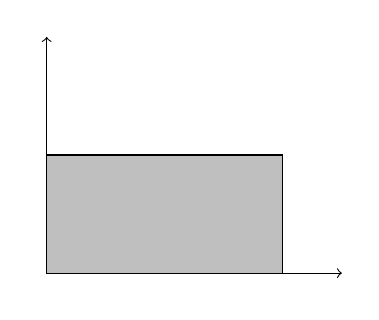
\begin{tikzpicture}[
		fatline/.style={>=latex,draw=blue,fill=blue},
		axis/.style={black,font=\small},
		linebase/.style={fill=lightgray},
		scale= 3
	]
		\draw[axis,->] (0,0) -- +(0,1) node[left] {$\uspeed$};
		\draw[axis,->] (0,0) -- +(1.25,0) node[below] {$\utime$};
		\draw[draw=black, fill=lightgray] (0, 0) rectangle(1,0.5);
	\end{tikzpicture}
	\caption{Flatarmálið undir grafinu gefur vegalengdina sem hefur verið ferðast.}
\end{figure}
%
\begin{figure}[!ht]
	\label{motion1d:fig:speedtimeareanonlinear}
	\centering
%	\includegraphics[width=0.25\textwidth]{./pictures/motion/motion_speed_time_nonlinear.eps}
	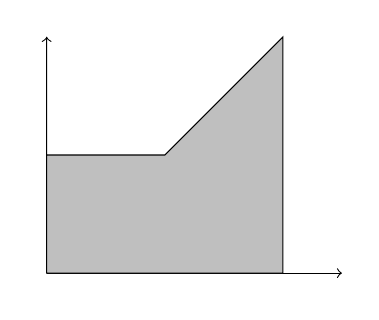
\begin{tikzpicture}[
		fatline/.style={>=latex,draw=blue,fill=blue},
		axis/.style={black,font=\small},
		linebase/.style={fill=lightgray},
		scale= 3
	]
		\draw[axis,->] (0,0) -- +(0,1) node[left] {$\uspeed$};
		\draw[axis,->] (0,0) -- +(1.25,0) node[below] {$\utime$};
		\draw[draw=black, fill=lightgray] (0, 0.5) -- ++(0.5,0) -- ++(0.5,0.5) 
			-- ++(0, -1) -- ++ (-1, 0) -- ++(0,1);
	\end{tikzpicture}
	\caption{Þrátt fyrir hraðabreytingu seinna meir á ferlinum gildir ennþá að
		flatarmálið undir graftinu gefur vegalengdina sem hefur verið ferðast,
		það getur oft orðið talsvert flókið að finna flatarmálið á hraða-tíma
		gröfum.}
\end{figure}
%
Sem sagt er hægt að meta hversu langt hlutur ferðast einunigs útfrá hraða-tíma
gröfum, hins vegar gildir \emph{ekki} það sama um stöðu-tíma gröf. Það sem við 
getum útleitt með hraða-grafi fyrir hlut sem hefur sömu hröðun (jöfn
hröðun) er vegalengdin sem er búið að ferðast, 
sjá mynd \ref{motion1d:fig:speedtimeconstaccle}. Sem er hægt að
setja sem jöfnu
\begin{equation}
	\Delta \ulengths = \uspeed_\text{byr} \utime 
		+ \frac{1}{2} \left(\uspeed_\text{loka} - \uspeed_\text{byr} \right) \utime
		= \uspeed_\text{byr} \utime + \Delta \uspeed \cdot \utime
\end{equation}
eða líka hægt að umskrifa til að vera
\begin{equation} \label{motion1d:eqn:constacceletime}
	\Delta \ulengths = \uspeed_\text{byr} \utime 
		+ \frac{1}{2} \uaccelea \utime^2
\end{equation}
sem er líka nefnd oft stöðujafna. 
\begin{figure}[!ht]
	\centering
	%\includegraphics[width=0.25\textwidth]{./pictures/motion/motion_speed_time_increasing.eps}
	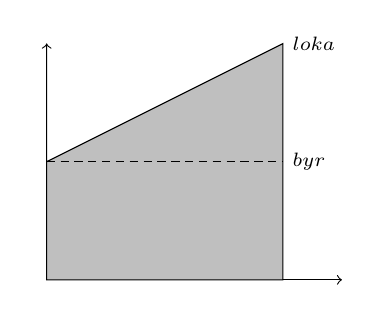
\begin{tikzpicture}[
		fatline/.style={>=latex,draw=blue,fill=blue},
		axis/.style={black,font=\small},
		linebase/.style={fill=lightgray},
		scale= 3
	]
		\draw[axis,->] (0,0) -- +(0,1) node[left] {$\uspeed$};
		\draw[axis,->] (0,0) -- +(1.25,0) node[below] {$\utime$};
		\draw[draw=black, fill=lightgray] (0, 0.5) -- ++(1.0,0.5) 
			-- ++(0, -1) -- ++ (-1, 0) -- ++(0,1);
		\draw[] (0,0) ++(1,1) node[right] {$\uspeed_\text{loka}$};
		\draw[densely dashed, draw=black] 
			(0,0.5) -- ++(1,0) node[right] {$\uspeed_\text{byr}$};
	\end{tikzpicture}
	\caption{Hérna sést hvernig hægt er að deila hraða-tíma grafi í þríhyrning
		og ferhyrning.}
	\label{motion1d:fig:speedtimeconstaccle}
\end{figure}
%
\begin{formalexample}
Bíll er á $\SI{54}{\km\per\hour}$ 
hraða, bíllinn bremsar niður í  $\SI{18}{\km\per\hour}$
hraða og það tekur $\SI{3.2}{\s}$. 
Hversu langt ferðast bíllinn á meðan hann er að bremsa?
\\[4 ex]
Byrjum á því að breyta í SI-einingar, 
$\SI{54}{\km\per\hour} = \SI{15}{\m\per\s}$
og $\SI{18}{\km\per\hour} = \SI{5}{\m\per\s}$. 
Við nýtum
\begin{align*}
	\Delta\ulengths & =  \uspeed_\text{byr} \utime 
			+ \frac{1}{2} \left(\uspeed_\text{loka} - \uspeed_\text{byr} \right) \utime
			\\
		& = \SI{15}{\m\per\s} \times \SI{3.2}{\s}
			+ \frac{1}{2} \times
				\left(
					\SI{5}{\m\per\s} - \SI{15}{\m\per\s} 
				\right) \times \SI{3.2}{\s}
			\\
		& = \SI{48}{\m} - \SI{16}{\m} \\
		& = \SI{32}{\m}
\end{align*}
\end{formalexample}
%
\begin{formalexample}
Bíll er á $\SI{54}{\km\per\hour}$ hraða, bíllinn eykur hraða sinn með hröðuninni
$\SI{3}{\m\per\s\squared}$ í $\SI{3.4}{\s}$.  
Hversu langt ferðast bíllinn á meðan hann eykur hraða sinn?
\\[4 ex]
Byrjum á því að breyta í SI-einingar, 
$\SI{54}{\km\per\hour} = \SI{15}{\m\per\s}$.
Við nýtum
\[
	\Delta\ulengths = \uspeed_\text{byr} \utime 
			+ \frac{1}{2} \uaccelea \utime
		= \SI{15}{\m\per\s} \times \SI{3.4}{\s}
			+ \frac{1}{2} \times 
				\SI{3}{\m\per\s\squared}
				\times \left( \SI{3.4}{\s} \right)^2
		= \SI{69.4}{\m}
\]
\end{formalexample}

\section{Hraðabreytingar og hröðun}
Þegar jöfn hröðun á sér stað, þá er hægt lýsa breytingunni án þess að nota
tíma sem lýsingu. Tíminn sem tekur fyrir hlut að auka hraða sinn jafnt er
\[
	\uspeed_\text{loka} = \uspeed_\text{byrjun} + \uaccelea \Delta\utime
		\Leftrightarrow
		\Delta\utime = \frac{\uspeed_\text{loka} - \uspeed_\text{byr}}{\uaccelea}
\]
ef við setjum þessa stærð inní stöðujöfnuna~\ref{motion1d:eqn:constacceletime} 
fæst
\begin{align*}
	\Delta\ulengths &= \uspeed_\text{byr} \utime 
		+ \frac{1}{2} \uaccelea \utime^2 
		&&\Leftrightarrow \\
	\Delta\ulengths &= \uspeed_\text{byr} \frac{\uspeed_\text{loka} - \uspeed_\text{byr}}{\uaccelea}
		+ \frac{1}{2} \uaccelea \left(\frac{\uspeed_\text{loka} - \uspeed_\text{byr}}{\uaccelea}\right)^2 
		&&\Leftrightarrow \\
	\Delta\ulengths &=  \frac{\uspeed_\text{loka}\uspeed_\text{byr} - \uspeed_\text{byr}^2}{\uaccelea}
		+ \frac{\left(\uspeed_\text{loka} - \uspeed_\text{byr}\right)^2}{2\uaccelea} 
		&&\Leftrightarrow \\
	2\uaccelea \Delta\ulengths &=  2\uspeed_\text{loka}\uspeed_\text{byr} - 2\uspeed_\text{byr}^2
		+ \left(\uspeed_\text{loka} - \uspeed_\text{byr}\right)^2
		&&\Leftrightarrow \\
	2\uaccelea \Delta\ulengths &=  2\uspeed_\text{loka}\uspeed_\text{byr} - 2\uspeed_\text{byr}^2
		+ \uspeed_\text{loka}^2 - 2\uspeed_\text{loka}\uspeed_\text{byr} + \uspeed_\text{byr}^2
		&&\Leftrightarrow \\
	2\uaccelea \Delta\ulengths &=  \uspeed_\text{loka}^2 - \uspeed_\text{byr}^2
\end{align*}
þeas. við höfum þá jöfnuna
\begin{equation} \label{motion:eqn:speedacceledist}
	2\uaccelea \Delta\ulengths =  \uspeed_\text{loka}^2 - \uspeed_\text{byr}^2
\end{equation}
sem getur lýst hraða, hröðun eða vegalengd hluta undir jafnri hröðun.
%
\begin{formalexample}
Bíll er á $\SI{54}{\km\per\hour}$ hraða, bíllinn eykur hraða sinn með hröðuninni
$\SI{3}{\m\per\s\squared}$ uppí hraðan $\SI{90}{\km\per\hour}$.  
Hversu langt ferðast bíllinn á meðan hann eykur hraða sinn?
\\[4 ex]
Byrjum á því að breyta í SI-einingar, 
$\SI{54}{\km\per\hour} = \SI{15}{\m\per\s}$ og
$\SI{90}{\km\per\hour} = \SI{25}{\m\per\s}$
Við umskrifum \ref{motion:eqn:speedacceledist} til að vera
\[
	2\uaccelea \Delta\ulengths =  \uspeed_\text{loka}^2 - \uspeed_\text{byr}^2
		\Leftrightarrow
		\Delta\ulengths = \frac{\uspeed_\text{loka}^2 - \uspeed_\text{byr}^2}{2\uaccelea}
			= 
				\frac{
					\left( \SI{25}{\m\per\s} \right)^2 
					- \left( \SI{15}{\m\per\s} \right)^2
					}{
					\num{2} \times \SI{3}{\m\per\s\squared}
					}
			= \SI{66.7}{\m}
\]
\end{formalexample}

\section[Línulegar jöfnur]{Hraði og línulegar jöfnur}
Hægt er að setja upp sett af línulegum jöfnum til að lýsa því hvað það tekur
langan tíma fyrir hluti að ná hvort öðru, t.d. bíll sem tekur frammúr öðrum bíl.
Til að lýsa því þá verður staðsetning hvers hlutar gefin með
\[
	\ulengths_\text{loka} = \uspeed \Delta\utime + \ulengths_\text{byrjun}
\]
gott er að muna að $\Delta \ulengths = \ulengths_\text{loka} 
- \ulengths_\text{byrjun}$.
Sem er staðsetning eins hlutarins, þá er hægt að setja upp tvær jöfnur
\begin{align*}
	\ulengths_\text{loka,A} &= \uspeed_\text{A} \Delta\utime 
		+ \ulengths_\text{byrjun,A} \\
	\ulengths_\text{loka,B} &= \uspeed_\text{B} \Delta\utime 
		+ \ulengths_\text{byrjun,B}
\end{align*}
báðar jöfnunar hafa sameiginlegan tíma sem er hægt að nýta til að leysa út eða tengja saman.
Fyrir lengra komna er hægt að sjá þessa sem fylki í hliðarrúmi%
~\footnote{S.s.  $\vec{\ulengths}_\text{loka} 
= \vec{\uspeed} \cdot \Delta\utime + \vec{\ulengths}_\text{byrjun} $}.
Það eru til nokkrar útfærslur á því hvernig hægt er að leysa þessar jöfnur.

\begin{formalexample}
Tveir bílar ferðast með jöfnum hraða, bíll A ferðast á $\SI{20}{\m\per\s}$ og 
bíll B ferðast með $\SI{15}{\m\per\s}$, bíll B er með $\SI{80}{\m}$ 
forskot miðað við A.
Hversu langan tíma tekur það fyrir bíl A að taka frammúr bíl B?
\\[4 ex]
Báðir bílarnir hafa staðsetningu miðað við núllpunkt bíls A til að vera
\begin{align*}
	\ulengths_\text{loka,A} &= 
		\SI{20}{\m\per\s} \times \Delta\utime + \SI{0}{\m} \\
	\ulengths_\text{loka,B} &= 
		\SI{15}{\m\per\s} \times \Delta\utime + \SI{80}{\m}
\end{align*}
þegar bíll A nær bíl B þá er staðsetning beggja sú sama
\begin{align*}
	\ulengths_\text{loka,A} &= \ulengths_\text{loka,B}\\
	\SI{20}{\m\per\s} \times \Delta\utime + \SI{0}{\m}
		&= \SI{15}{\m\per\s} \times \Delta\utime + \SI{80}{\m}\\
	\SI{20}{\m\per\s} \times \Delta\utime 
		- \SI{15}{\m\per\s} \times \Delta\utime 
		&=  \SI{80}{\m} \\
	\left( 
		\SI{20}{\m\per\s} - \SI{15}{\m\per\s} \right) \Delta\utime 
			&= \SI{80}{\m} \\
	\left( \SI{5}{\m\per\s} \right) \Delta\utime &=  \SI{80}{\m} \\
	\Delta\utime &=  \frac{ \SI{80}{\m} }{ \SI{5}{\m\per\s} }\\
		&=  \SI{16}{\s}
\end{align*}
\end{formalexample}

\begin{formalexample}
Bíll A bíður á ljósum og bíll B fer frammhjá með hraðanum $\SI{15}{\m\per\s}$, 
bíll A hefur hröðunina $\SI{2}{\m\per\s\squared}$ og hraðar sér upp í hraðan 
$\SI{20}{\m\per\s}$, hversu lengi er bíll A að ná bíl B?
\\[4 ex]
Til að byrja með er gott að athuga hvort að bíll A nær bíl B á meðan hröðun stendur,
það tekur bíl A að hraða sér frá kyrrstöðu upp í $\SI{20}{\m\per\s}$ nákvæmlega 
$\SI{10}{\s}$. Þá hafa bílarnir ferðast
\begin{align*}
	\ulengths_\text{hröð,A} 
		&= \frac{1}{2} \times \SI{2}{\m\per\s\squared} \times 
			\left( \SI{10}{\s} \right)^2 = \SI{100}{\m} \\
	\ulengths_\text{hröð,B} 
		&= \SI{15}{\m\per\s} \times \SI{10}{\s} 
		= \SI{150}{\m}
\end{align*}
báðir bílarnir hafa staðsetningu miðað við núllpunkt bíls A til að vera
\begin{align*}
	\ulengths_\text{loka,A} 
		&= \SI{20}{\m\per\s} \times \Delta\utime + \SI{100}{\m} \\
	\ulengths_\text{loka,B} 
		&= \SI{15}{\m\per\s} \times \Delta\utime + \SI{150}{\m}
\end{align*}
þegar bíll A nær bíl B þá er staðsetning beggja sú sama
\begin{align*}
	\ulengths_\text{loka,A} &= \ulengths_\text{loka,B}\\
	\SI{20}{\m\per\s} \times \Delta\utime + \SI{100}{\m}
		&= \SI{15}{\m\per\s} \times \Delta\utime + \SI{150}{\m} \\
	\SI{20}{\m\per\s} \times \Delta\utime 
		- \SI{15}{\m\per\s} \times \Delta\utime 
		&= \SI{50}{\m} \\
	\left( 
		\SI{20}{\m\per\s} - \SI{15}{\m\per\s} 
	\right) \Delta\utime 
		&=  \SI{50}{\m} \\
	\left( \SI{5}{\m\per\s} \right) \Delta\utime 
		&=  \SI{50}{\m} \\
	\Delta\utime 
		&=  \frac{ \SI{50}{\m} }{ \SI{5}{\m\per\s} }\\
		&=  \SI{10}{\s}
\end{align*}
þá er samanlagður tími sem er í að ná bíl B
\[
	\Delta\utime = \Delta\utime_\text{hröðun} + \Delta\utime_\text{jafn}
		= \SI{10}{\s} + \SI{10}{\s} = \SI{20}{\s}
\]
\end{formalexample}
